\section{Apparatus}

As detailed in the section on the measurement scheme, \CENTREX\ follows the
design of a conventional molecular beam experiment. Fig.~\ref{entire} displays
an outline of the entire apparatus, Table~\ref{parametertable} contains key
parameter values, and the following paragraphs give information about its
construction. \todo{Say who did what part of the apparatus, perhaps as a table,
or in an appendix.}

\begin{figure*}[b!]
    \begin{overpic}[width=\textwidth,unit=1mm]{figs/entire.pdf}
            \put(22,72){beam source}
            \put(28,68){gate valve}
            \put(2,18.5){bellows}
            \put(29,61){\parbox{2.5cm}{\linespread{.9}rotational\\cooling}}
            \put(58,71){state prep 1}
            \put(56,62){electrostatic quadruple lens}
            \put(77,55){gate valve}
            \put(83,47){interaction region}
            \put(128.6,56){gate valve}
            \put(129,62){state projection}
            \put(129,70.5){detection chamber}
            \put(73,20){state prep 2}
            \put(73,26){bellows}
            \put(132,14){bellows}
            \put(0,  4){0}
            \put(13, 4){0.63}
            \put(25, 4){1.12}
            \put(33, 4){1.42}
            \put(50, 4){2.08}
            \put(63, 4){2.59}
            \put(150,4){6.09}
            \put(163,4){6.57}
            \put(176,4){7.08}
    \end{overpic}
    \caption{Overview of the \CENTREX\ beamline without the magnetic shield
    around the interaction region. Note that the second state-preparation
    region, and the detection chamber, have not yet been designed. The
    horizontal ordinate is given in meters.} \label{entire}
\end{figure*}

\begin{table}[!htb]
    %\makebox[\columnwidth][c]{%
    \begin{tabu} to \columnwidth {@{}rcX[c]l@{}}
        \toprule
        Parameter & Sym. & Value & Units \\
        \midrule
        \multicolumn{3}{@{}l}{\textit{Beam source:}}\\
           total source intensity       & $I_0$             & $10^{10-12}$           & mol./s/sr/state  \\
           average beam velocity        & $v_\text{CM}$     & $184\pm17$             & m/s              \\
           beam velocity spread         & $\alpha$          & $16\pm1$           & m/s              \\
           rotational temperature       & $T_\text{rot}$    & $6.5\pm0.2$            & K                \\
           vibrational temperature      & $T_\text{vib}$    & 8                      & K                \\
           pulse duration               & $\Delta t$        & 20                     & ms               \\
           beam diameter                & $d_\text{beam}$   & 2.5                    & cm               \\
           nozzle diameter              & $d_\text{noz}$    & \nicefrac{1}{4}        & in               \\
           nozzle to detector dist.     & $L_\text{nd}$     & 6.45                   & m                \\
        \\\multicolumn{3}{@{}l}{\textit{Quadrupole lens:}}\\
           quadrupole voltage           & $V_\text{quad}$   & $\pm30$                & kV               \\
           bore diameter                & $d_\text{quad}$   & 1.75                   & in               \\
           length                       & $L_\text{quad}$   & 60                     & cm               \\
        \\\multicolumn{3}{@{}l}{\textit{Interaction region:}}\\
           SOF coil frequency           & $f_0$             &                        & kHz              \\
           slope of SOF resonance       & $\d I/\d f$       & 0.094                  & 1/Hz             \\
           interaction region $E$ field & $E_\text{int}$    & $\pm30$                & kV               \\
           interaction region $B$ field & $B_\text{int}$    & $<10$                  & $\mu$G           \\
           SOF coil separation          & $L_\text{SOF}$    & 3                      & m                \\
           interaction time             & $T$               & 16                     & ms               \\
           resonance FWHM               & $\Delta f$        & 33.2                   & Hz               \\
           SOF coil width               & $d_\text{SOF}$    & 10                     & cm               \\
        \\\multicolumn{3}{@{}l}{\textit{Detection region:}}\\
           detection efficiency         & $\eta_\text{det}$ & 100~\%                 & ---              \\
           detection rate               & $R_\text{det}$    & $2\cdot10^9$           & mol./sec         \\
           source-detector distance     & $L_\text{sd}$     & $594\pm10$             & cm               \\
           background count             & $I_\text{b}$      & \todo{???}             & mol./sec         \\
           detection area               & $A_\text{det}$    & \todo{???}             & mm$^2$           \\
           signal to noise ratio        & SNR               & \todo{???}             & ---              \\
           fringe contrast              & $C_\text{f}$      & \todo{???}             & ---              \\
           \bottomrule
    \end{tabu}%}
    \caption{Key parameters of the \CENTREX\ experiment.}
    \label{parametertable}
\end{table}

\subsection{Control software}

The experimental parameters are monitored and controlled using a range of
devices. Most of these have already been integrated into a central data
acquisition (\DAQ) system. At present, the latter consists of a single highly
configurable Python program running on all computers attached to the experiment,
communicating with the devices connected to the computer and writing the
obtained data to the local disk. In the future, we intend to set up a common
data and backup server to deal with the greatly increased data generation rate
once the entire apparatus is up and running.

The program's code is divided between classes that make up the graphical user
interface (\GUI), and control classes which make use of driver classes to
communicate with physical instruments. In addition, all program configuration is
contained in \verb`.ini` files in subdirectories of the so-called \verb`config`
directory, allowing for simple modification and extension of the \DAQ\ system
without changing the main program code. This configuration is loaded into the
relevant \verb`Config` class.

The user controls the devices through the \verb`ControlGUI`, which is a canvas
for control of recording and external devices. The information in device config
files is automatically read and translated into usable controls that appear in
the \GUI. Underneath the graphical interface, several classes implement the
program's functionality:

(1) \verb`Device` objects run each within its own thread, instantiate device
drivers, and poll devices at regular intervals for data as well as check for
normal operation insofar as supported by the driver, pushing this information
into data and events queues specific to each device. In addition, these objects
serve as an unified abstract interface to all the drivers and related
information, especially through the \verb`config` member (of type
\verb`DeviceConfig`).

(2) \verb`Monitoring`: While the \verb`Device` objects collect information from
the physical devices, they neither record it nor notify the user in case of any
abnormal condition. Thus the main program instantiates one \verb`Monitoring`
object to read some of the data, display it in the main interface, and send it
to an external central database.

(3) The \verb`HDF_writer` stores the data collected by \verb`Device` objects to
an file for future reference and analysis. The files are of Hierarchical Data
Format (\HDF), version 5 format \cite{doecode_9801}, a portable, cross-platform
format that provides \API s for commonly scientific computing languages. The
format is extensible, open, and structured, allowing storage of data and its
description in terms of arbitrary attributes, column names, and groups.

(4) \verb`Config` classes serve to organize access to program, device, or plot
configuration. Thus, instead of having classes pass ad hoc pieces of information
between each other, they set an appropriately-named attribute of the relevant
\verb`Config` class. The latter in term only allows to set the attributes that
have been declared previously. This enables the programmer to have a clear
overview of what configuration parameters exist by simply inspecting the
relevant \verb`Config` class.

The program is thus generic enough to make it easy to add capabilities to
control any number of new devices by simply (1) writing a device driver, and (2)
a device config file. Drivers are classes inside the Python modules, such that
instantiating the driver class is the abstract representation of opening a
connection to a physical device. In addition, a driver class provides a
\verb`ReadValue()` method that implements the particulars about how reading data
works, and should return a list of values, consistent with the \verb`dtype` and
\verb`shape` of the device as specified in the constructor. The driver must also
provide a function \verb`GetWarnings()` that is be called at regular intervals
to populate the list of \verb`warnings`. This function can check for the device
parameters are within normal ranges, or simply do nothing if appropriate.

Upon starting, the program reads the main config file that defines general
program settings; the values are read by the instance of \verb`ProgramConfig`
class. Device configurations are read from \verb`.ini` files in the chosen
directory. Thus choosing a different directory allows for a different set of
devices or device configurations to be loaded. These files define the controls
that to appear on the screen for each instance of a device, the driver commands
called from these controls, and their default values.

The device \verb`.ini` file should specify whether the device is a slow or a
fast device.  A slow device is expected to return only a few values each time
its \verb`ReadValue()` is called, and thus requires a single dataset to contain
all the data. A fast device can return thousands or millions of datapoints each
time it is polled, together with metadata that describes this particular set of
values. Thus, the program creates a new dataset for each invocation of
\verb`ReadValue()` of a fast device.

\subsection{Beam source}
\label{sect:beamsource}

The beam source works by ablation of a solid sample of TlF held at cryogenic
temperatures in a thermally shielded vacuum chamber. The ablated particles are
expelled from the ablation cell by a flow of cold neon buffer gas. The design
has been adapted from the beam source used in ref.~\cite{barry2011bright} with
significant modifications.

The ablation cell is a 1.500~in high cuboid with top and bottom square faces
with a 2.000~in side, machined out of \OFHC\ copper (Cu 101). The internal
volume consists of two intersecting cylinders of diameter $d=1.150$~in and
length $L=2.000$~in. According to a formula known to Archimedes
\cite{moore1974symmetrical}, the volume common to the two cylinders is
$\frac{2}{3}d^3$, making the internal cell volume for two cylinders to be
$V=2L\pi\frac{d^2}{4}-\frac{2}{3}d^3\approx3.14\inches^3$. The actual internal
volume is slightly larger than that due to the way windows are attached to the
cell.

Three of the four circular openings in the cell are closed with fused silica
windows, while the forth is covered by a thin plate of \OFHC\ copper (0.050~in
thickness) with a \nicefrac{1}{4}~in aperture as the molecular beam exit nozzle.
Unlike similar beam sources, the exit aperture is \emph{not} followed by a
conical collimator, since we found it interferes with the collision-mediated
beam thermalization processes (an effect highly sensitive to the exact
placement, shape, and dimensions of the collimator). In order to protect the
window through which the ablation laser (Fig.~\ref{ablationLaser}) enters from
the immediate ablation by-products, the window is offset by a 3~in-long
`snorkel', a cylinder of outer diameter 1.250~in, and an hole with internal
diam. of 0.9~in going through the entire length of the piece. The cylinder is
terminated on one end in a way that allows attaching it to the cell, and on
another by a fitting for the window.

\begin{figure}
    \centering
    \def\svgwidth{1\columnwidth}
    \input{figs/svg/lasers1.pdf_tex}
    \caption{The ablation laser for the beam source is a pulsed Nd:YAG,
    provinding 4~ns pulses of maximum energy 130~mJ at max.\ 50~Hz (Nano LG
    130-50 by Litron Lasers Ltd, UK). In beam source tests, we have commonly run
    it such that the pulse energy is approx.\ 35~mJ, at a repetition rate of
    5--10~Hz. The photodiode receives a small amount of light split off the main
    beam, and is used for monitoring the laser power. [Drawing by O. Grasdijk]}
    \label{ablationLaser}
\end{figure}

The cell opening opposite the ablation laser is covered by the target holder, a
copper piece machined so as to contain a volume of solid TlF. The targets are
prepared in a separate chamber by filling them with powdered 99~\%\ pure
thallium(I) fluoride (supplied by Strem Chemicals, Newburyport, MA, under
product number 93-8106) and heating to a temperature just above the melting
point 327\degC. In the early stages of beam characterization, the target holder
had a small (\nicefrac{1}{4}~in diam.) opening, covered by another snorkel and
window, to allow for absorption probing the TlF population in the cell.

The buffer gas is 99.999~\% pure neon, supplied by TechAir (Naugatuck, CT).
Outside the vacuum chamber, neon flow is moderated by a 412 series dual-stage
pressure regulator (Concoa, Virginia Beach, VA), and a mass-flow controller (MKS
Instruments, Andover, MA; part number 1179C00212CR1AV) that allows up to
100~sccm of flow. The gas is fed from the bottle using \nicefrac{1}{4}~in copper
tubing.

The opening opposite the cell exit nozzle has a 0.375~in opening that allow
optical access along the direction of the molecular beam. In addition,
perpendicularly through the same hole, the neon buffer gas enters the cell
through a \nicefrac{1}{16}~in opening. The gas enters the beam source vacuum
chamber via a \KF\oldstylenums{40}-to-\VCR\ (\nicefrac{1}{8}~in) feedthrough
(Accu-Glass Products, Valencia, CA; part number 113030). To thermally separate
the room-temperature vacuum chamber from the cryogenic parts, the connection is
insulated by smooth-bore seamless 304 stainless steel tubing, \nicefrac{1}{8}~in
OD, 0.02~in wall thickness (McMaster-Carr Supply Company, Elmhurst, IL; part
number 89895K711). The stainless tubing is approx.\ 3~ft long, wound in a coil
(approx.\ diam. 3~in) to save space. The gas line is thermally connected to the
40~K shield by flowing through \nicefrac{1}{8}~in copper tubing wound around and
brazed on a \nicefrac{3}{4}~in-diam.\ copper bobbin that is fixed to the 40~K
shield with a threaded rod. Another similar coil of stainless tubing limits heat
flow from the 40~K shield to the cell. Finally, the neon thermalizes to the cell
temperature by flowing through an approx.\ 6~in-long segment of
\nicefrac{1}{8}~in copper tubing that is brazed to the piece that attaches to
the cell.

The cell is screwed onto the cold stage of the PT815 cryocooler (made by
Cryomech Inc., Syracuse, NY). The cell is shielded from ambient thermal
radiation by a two-state heat shield. The outer shield, made of aluminum 1100,
hangs from the top plate of the vacuum chamber on stainless threaded rods and
consists of a frame with removable covering plates and is thermally connected to
the `warm' stages (approx.\ 40~K) of both pulse-tube cryocoolers. The inner
shield, hanging from the outer one on four \nicefrac{1}{4}~in stainless threaded
rods, is made of \nicefrac{1}{4}~in thick Cu101 plates, and is connected to the
cold stage of the colder PT415 cooler, which cools it to approx. 4--5~K. The 4~K
shield has bare openings for optical and molecular access, while the optical
ports in the 40~K shield are blocked with loosely attached windows to limit the
buffer gas escaping into to rest of the apparatus. The cell--cryocooler thermal
links are done via flexible copper braids to prevent damage from unmatched
thermal expansion coefficients.

For control of cell temperature, a number of 10--25~$\Omega$ resistors are
attached directly to the cell and heated directly with standard laboratory power
supply, or controlled in a \PID\ loop using the CTC100 cryogenic temperature
controller (Stanford Research Systems, Sunnyvale, CA). The same controller gets
temperature input from the silicon diode sensors (DT-670 from Lake Shore
Cryotronics, Inc., Westerville, OH) located on the cell gas-input nozzle, cell
top plate (target side), 4~K and 16~K pulse tube warm stages. The other eight
sensors, recorded by the model 218 temperature monitor from Lake Shore
Cryotronics, are located on the cell back snorkel, 4~K shield top plate, 40~K
shield top plate, 4~K pulse tube cold head, cell top plate, 4~K shield bottom
plate, 40~K shield bottom plate, and the 16~K pulse tube cold head. These eight
sensors' wires are fed through the vacuum chamber using two 25-pin feedthroughs
(Accu-Glass p.n.\ 100225), with corresponding vacuum-side PEEK female D-sub
connectors (Accu-Glass p.n.\ 100460) for ease of disconnecting.

\begin{figure*}
    \centering
    \def\svgwidth{\textwidth}
    \input{figs/svg/lasers2.pdf_tex}
    \caption{UV laser system (see text). \part{a} Cs reference laser. \part{b}
    Transfer scanning cavity frequency lock. \part{c} Two-state second harmonic
    generation (\SHG). [Drawings by O. Grasdijk]}
    \label{lasers}
\end{figure*}

Cell windows are standard fused-silica \UV-grade windows (from Thorlabs, Newton,
NJ). The anti-reflect coatings, done at 271~nm (excited-to-ground molecular
transition) and 1064~nm (ablation laser) were done by Thin Film Lab (Milford,
PA). All removable mechanical connections are done by means of brass screws into
threaded holes, reinforced with stainless threaded inserts (Heli-Coil). All
gas-line connections are done with \VCR\ fittings brazed onto the copper or
stainless tubing. Where possible and desirable, metal-to-metal thermal
conductivity has been enhanced either with indium foil, or vacuum-compatible
grease (Apiezon N).

\subsection{Pumping system}

In addition to providing thermal isolation, the shields also serve as cryopumps,
lowering the pressure from $\sim10^{-6}$~torr, as can be reached by
turbomolecular pumps, to approx.\ $2\cdot10^{-8}$~torr. Pumping down from
atmospheric pressure is done with nXDS 6i and 10i dry scroll pumps (Edwards
Vacuum, UK) and HiPace 700M turbomolecular pumps (Pfeiffer Vacuum Technology AG,
Germany). Pressure is monitored with ionization vacuum gauges (IGM401 Hornet
from InstruTech LLC, Longmont, CO).

\subsection{Mounting structure}

The vacuum chambers that make up the beamline are mounted on a substructure
built out of 80/20 aluminum rails. The stands for all chambers but the
interaction region are placed on steel wheels that allow us to slide the chamber
out of the beamline perpendicularly (Fig.~\ref{transverse_rail}). This is
accomplished using a set of transverse rails (also quad-profile 80/20) which are
in turn connected to a longer rail that runs parallel to the beamline. The main
purpose of this system is to allow access to the inside of the interaction
region, such as to measure the internal magnetic fields, without having to move
the magnetic shield in which it is contained. (Moving the shield itself would
change the internal fields significantly, which would defeat the purpose of
moving it.) When the chambers do not need to be moved, they can be fixed in
place using connection plates that directly connect the stand to the transverse
rail.

\begin{figure}
   \centering
  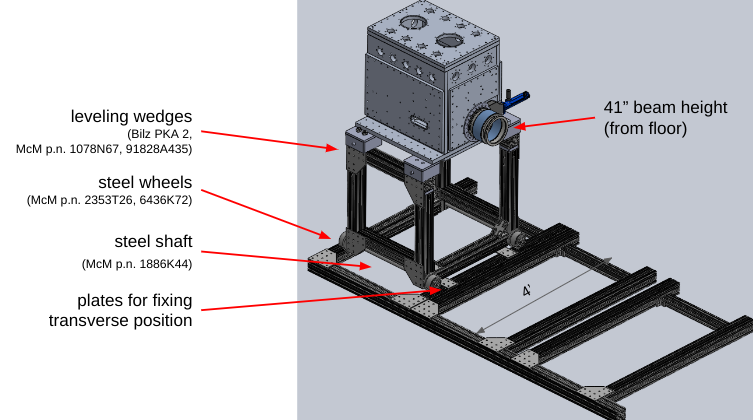
\includegraphics[width=\textwidth]{figs/todo/transverse_rail.png}
   \caption[Transverse rail mounting structure.]{Transverse rail mounting
    structure. Only the beam source is shown, but other chambers, with the
    exception of the interaction region, are to be mounted similarly.}
  \label{transverse_rail}
\end{figure}

\subsection{Laser system}

See Fig.~\ref{lasers} for a diagram of the \UV\ laser system. It consists of
three systems working together to (1) provide a stable cesium reference line,
(2) lock an \IR\ seed laser to the reference, and (3) to quadruple the \IR\ into
a \UV\ beam that can be used to probe transitions in TlF, occuring around
271~nm. In order to provide separately-controllable laser frequencies, we have
three \SHG\ systems connected to two transfer lock cavities (one of them
currently under construction).

\paragraph{Cs lock}

The reference system is based on modulation transfer spectroscopy (\MTS), a
pump--probe technique resulting in sub-Doppler resolution for laser locking. An
\EOM\ modulates the pump beam (so as to cause sidebands to accompany the carrier
frequency) before it gets passed through a vapour cell. Modulation can appear on
the counterpropagating probe beam, passed through the same vapour, through the
interactions of the two beams with the atomic vapour. The interactions are an
example of four-wave mixing where two pump beam frequency components combine
with the probe beam, resulting in a sideband for the probe beam.
\cite{mccarron2008modulation}

In contrast, in frequency modulation spectroscopy (\FMS) only a single modulated
beam is passed through the sample and onto a detector. If the modulation
frequency is large compared with the spectral feature being probed, then the
laser (or \EOM) can be tuned such that only one sideband interacts with the
sample. In the absence of such an interaction, the \RF\ signal arising from the
beating of one sideband with the carrier cancels that arising from the other
sideband. When this balance is upset by phase or amplitude changes in one
sideband, and a background-free signal results. \cite{bjorklund1980frequency}

Following ref.~\cite{zi2017laser}, the beam sourced from the diode laser (DL pro
850, Toptica, Germany) is split off for transfer cavities with two polarizing
beam splitters (with the two half-wave plates controlling the amount of light
sent to each transfer cavity beam). The remaining beam is split by the
acousto-optic modulator (\AOM) (AOMO 3080-122 830NM from Gooch \&\ Housego, UK)
with 80~MHz center frequency, AR-coated for operation at 780--850~nm, into a
pump and probe beam, the pump having about twice the power of the probe. (The
\AOM\ also eliminates trouble from backreflection from the Cs cell, or
photodiodes.) The pump beam is phase-modulated by the custom-built \EOM\
(Thorlabs Inc.) at 3~MHz before being led through the cesium quartz cell
(Thorlabs GC19075-CS, diam.\ 19~mm, length 75~mm), magnetically shielded to the
milligauss level in a 6~in-long, 2~in inner diam.\, three-layer concentric
mu-metal shield (modified ZG-203 from Magnetic Shield Corporation, Bensenville,
IL). 

The \MTS\ signal is detected by the photodiode (we have not found it necessary
to make use of the \FMS), and mixed with the \EOM\ driving frequency to obtain
an error signal used inside the laser controller (Toptica DLC pro) to stabilize
the laser diode current and the piezo-controlled cavity, and lock it to the
$F=4\to5$ transition in the hyperfine structure of the cesium D$_2$ line,
occuring at 852.35641~nm \cite{steck2003cesium}. However, as the Cs reference is
only used to set the scale in the \FSR\ of the transfer cavity, the choice of
the hyperfine level is not important---GHz differences cause differences
negligible compared to the $\approx0.5$~MHz stability required for the \IR\
science lasers.

\paragraph{Transfer cavity}

The Fabry--P\'erot interferometer (Toptica FPI 100) with free spectral range
(\FSR) 1~GHz is locked to the cesium reference (master) laser. Up to two slave
lasers can be used in this scheme, one for each of the two orthogonal
polarizations, while the master can be distinguished by its different wavelength
and separated away with a dichroic mirror. The cavity length is modulated by
slighly more than one \FSR\ to scan over the transmission peaks. The timing
difference between the master and slave peaks is then fed to a \PID\ loop to
lock the slave frequency.

\paragraph{Second harmonic generation}

The \IR\ beam at 1087~nm is generated by the Koheras Basik fiber laser seed and
amplified to $\approx2$~W by the Koheras Boostik Fiber Laser (both devices by
NKT Photonics A/S, Denmark). A small amount of power is split off for the
wavemeter (671A by Bristol Instruments, Rochester, NY), which allows for a
measurement of the absolute laser frequency to within 50~MHz. The rest of the
beam is modulated by an \EOM\ and passed through a bowtie-configuration cavity
(built by K. Wenz at Columbia, NY) containing a ppKTP crystal that generates up
to 1~W of green light at 543.5~nm. The green beam is coupled into a fiber and
delivered to a second \SHG\ system (Toptica SHG pro) with a similar
configuration. A BBO crystal is used for frequency doubling, resulting in
$\approx70$~mW of \UV\ (271.7~nm).

To counteract the cavity length changes due to temperature and pressure
variations, one of the cavity mirrors is attached to a piezo actuator. Using the
Pound--Drever-Hall technique (\PDH), the cavity photodiode signal is mixed with
the \EOM\ driving frequency in order to extract a sensitive error signal that
can be used to \PID-control the piezo actuator. \cite{drever1983laser} The \UV\
lock is done with a commercial analog setup (Toptica PDH 110, PID 100, and FALC
110), while for the green cavities we are transitioning to a home-built system,
based on the Red Pitaya STEMlab \FPGA\ board.

\begin{figure}
    \makebox[\columnwidth][c]{%
        \small
        \usetikzlibrary{shapes.geometric}
\tikzstyle{block} = [rectangle, draw, text width=3em, text centered, rounded corners, minimum height=3em]
\tikzstyle{cross} = [draw,circle,minimum width=1 cm,path picture={ 
  \draw[black]
  (path picture bounding box.south east) -- (path picture bounding box.north west) (path picture bounding box.south west) -- (path picture bounding box.north east);
  }]
\tikzstyle{amp} = [regular polygon, regular polygon sides=3, draw, text centered, shape border rotate=90]
\tikzstyle{arr} = [draw, -Latex]
\def\freqsize{\footnotesize}
\def\dy{.3cm}
\def\dyy{.8cm}
\def\dyyy{1.3cm}
\def\dx{0.7cm}
\def\dxx{1.5cm}

\begin{tikzpicture}
    \linespread{.9}

    % place nodes
    \node [block, text width=4em] (siggen)  {Signal\\generator};
    \node [cross, right = \dxx of siggen] (mix1)    {};
    \node [block, right = \dx of mix1]    (LP)      {Low pass};
    \node [cross, above = \dyy of LP]     (mix2)    {};
    \node [block, right = \dxx of mix2]   (HP)      {High pass};
    \node [block, below = \dy of siggen]  (agile)   {Freq.\\agile\\AWG};
    \node [block, below = \dyyy of HP, text width=6.5em]      (mult)    {$\times1$, 2 or 4\\freq.\ multiplier};
    \node [block, below = \dyyy of mult]   (SPDT)    {SPDT};
    \node [below = \dy of SPDT]   (SPDT2)    {};
    \node [block, left = \dx of SPDT, text width=4.5em]     (OMT)     {orthomode\\transducer};
    \node [amp,   left = \dx of OMT]      (amp)     {amp};
    \node [block, left = \dx of amp]      (horn)    {horn};

    % connections
    \draw [arr] (siggen) -- node [above] {\freqsize 1 GHz} (mix1);
    \draw [arr] (siggen) |- node [above right] {\freqsize 12.65 GHz} (mix2);
    \draw [arr] (agile) -| node [above left] {\freqsize 200--300 MHz} (mix1);
    \draw [arr] (LP) -- node [right,text width=4.5em] {\freqsize 700 to\\800 MHz} (mix2);
    \draw [arr] (mix1) -- (LP);
    \draw [arr] (mix2) -- (HP);
    \draw [arr] (HP) --  node[xshift=2.5em, text width=7.5em, text centered] {\freqsize 13.35 GHz\\to\\13.45 GHz} (mult);
    \draw [arr] (mult) -- (SPDT);
    \draw [arr] (SPDT) -- (OMT);
    \draw (SPDT) -- (SPDT2.south);
    \draw [arr] (SPDT2.south) -| (OMT);
    \draw [arr] (OMT) -- (amp);
    \draw [arr] (amp) -- (horn);
\end{tikzpicture}

    }
    \caption{The principle behing frequency-agile rotational cooling microwave
    generation. The frequencies are shown assuming the $\times1,2$ multipliers
    for a horn output of 13.4 and 26.8~GHz. For 40.1~GHz, the system is adjusted
    to generate approx.\ 10~GHz (pre-multiplier).} \label{micro}
\end{figure}

\subsection{Rotational cooling}
\label{sect:rotcool}

We designed a custom aluminum vacuum chamber to allow access for the molecular
beam, \UV\ laser, and microwaves as required by the rotational cooling scheme.

The microwave system (see Fig.~\ref{micro}) is designed to provide up to three
microwave beams (at frequencies 13.4, 26.8, and 40.1~GHz, and power of order
0.1--1~W), each focused with a quasioptical lens built into the transmitting
antenna so as to position the beam waist in the center of the vacuum chamber. In
addition, the beams can be switched between either of the two orthogonal linear
polarizations at 1--2~MHz. In order to be able to separately address the
hyperfine levels in the molecular ground state, the frequency can be rapidly
adjusted by means of direct digital synthesis (\DDS).

The ability of an \RF\ system to resolve spectral features can be described in
terms of phase noise, defined as the ratio (in decibels) of the noise in a 1~Hz
bandwidth at a specified offset $f_m$, to the oscillator signal amplitude at
frequency $f_0$. In a microwave communications context, a local oscillator at
frequency $f_0$ is used to downconvert the desired signal $f_\text{D}$ to an
intermediate frequency $f_\text{IF}$. We want to know what is the maximum
allowable phase noise $L_\text{max}$ (in dBc/Hz) so that the downconversion of
an adjacent undesired (interference) signal $f_\text{ID}$ is suppressed by a
factor of $S$, called selectivity and expresssed in dB. The maximum phase noise
is \cite[eqn~13.50]{pozar2006microwave}
%
\[
    L_\text{max}=D-S-I-10\log(B),
\]
where $D$ is the desired signal level (dBm), $I$ is the undesired (interference)
signal level (dBm), and $B$ is the bandwidth (in Hz) of the intermediate
frequency.

To translate this into the language of atomic physics, the goal is no longer to
convert a signal down to IF, but rather to drive a transition at a specified
detuning without exciting adjacent transitions. The previously defined variables
acquire new meanings:
%
\begin{align*}
    f_0 &=\text{applied \RF\ frequency}\\
    f_\text{D} &=\text{desired transition frequency}\\
    f_\text{I} &=\text{frequency of a nearby unwanted transition}\\
    f_\text{IF} &=\text{detuning}
\end{align*}
%
Assuming the desired ($D$) and undesired ($I$) signals are both same strength,
and the signal linewidth (from molecular fly-through time) is $B\approx10^3$~Hz,
a 20~dB selectivity requires the phase noise to be smaller than $-50$~dBc/Hz.
This requirement is satisfied by both signal sources described below.

The \DDS\ source is AD9910 (Analog Devices Inc., Norwood, MA), outputting out to
approx.\ $f_\text{\DDS}=400$~MHz. The signal is mixed with a fixed $f_0=1$~GHz
wave generated by one of the outputs of the SynthHD Pro (WindFreak Technologies,
Holiday, FL). A low pass filter removes the sum component $f_\text{\DDS}+f_0$
and passes the difference, to be mixed with a $12.65$~GHz signal from the other
SynthHD output. In the second stage, a high-pass filter has to be used, passing
the sum of the frequencies, since the signal generator only goes up to 14~GHz.
This also filters out a strong sub-harmonic in the high-frequency SynthHD
output. (Two-stage mixing is required because of the difficulty in filtering out
one of the 100~MHz sidebands from a signal exceding 10~GHz.) The resulting
frequency-agile microwave signal is doubled or quadrupled if necessary,
amplified, power-split with an SPDT switch, and recombined in an orthomode
transducer before being led to the horn. The horns were custom engineered by
Sage Millimeter (now Eravant Inc., Torrance, CA) for spot-focusing the beam
energy onto the molecular beam.

\subsection{State preparation 1}

The design for the first state preparation region is currently under way.

\subsection{Electrostatic lens}

\todoit{Constructed by Oskari Timgren. TBD.}

\subsection{State preparation 2}

The second state preparation region has not yet been designed.

\subsection{Interaction region}

\todoit{Constructed at UMass. TBD.}

The coil setup is currently being designed. For a thorough uncertainty analysis,
the system will need the ability to apply small $B_z$ field in interaction
region, as well as small $B_y$ and $B_x$ and small gradients, such as $\d B_z/\d
x$.

\subsection{State projection and readout}

To be designed.
